% Compile from this directory with XeLaTeX (twice): xelatex report.tex
% Course format: Times New Roman 12 pt, 2.5 cm margins, single spacing, A4; 4 pages excluding references.
\documentclass[a4paper,12pt]{article}
\usepackage[margin=2.5cm]{geometry}
\usepackage{fontspec}
\setmainfont{Times New Roman}
\usepackage{amsmath,amssymb}
\usepackage{booktabs}
\usepackage{graphicx}
\usepackage[labelfont=bf,skip=3pt]{caption}
\usepackage[compact]{titlesec}
\titleformat{\section}{\bfseries}{\thesection}{0.5em}{}
\titlespacing*{\section}{0pt}{5pt}{1pt}
\usepackage[hidelinks]{hyperref}
\hypersetup{pdftitle={Where Should Capacity Count? Residual Transport and the Embedding Path in Neural Spectral Capacity},
  pdfsubject={CS5491 Project Report}}
\setlength{\parindent}{0pt}
\setlength{\parskip}{3pt}
\setlength{\textfloatsep}{6pt}
\setlength{\floatsep}{6pt}
\setlength{\abovedisplayskip}{2pt}
\setlength{\belowdisplayskip}{2pt}
\setlength{\tabcolsep}{4pt}
% Public build lists names only; submit.tex (private, not in the repository) adds IDs and email.
\ifdefined\UsePrivateTeam
  \input{team-private.tex}
\else
  \def\TeamMembers{Kaiwen Wang, Leao Wang, Lei Gao}
  \def\ContactEmail{}
\fi
\newcommand{\psimp}{\psi_{\mathrm{MP}}}

\begin{document}
\begin{center}
\textbf{Where Should Capacity Count? Residual Transport and the Embedding Path in Neural Spectral Capacity}\\
CS5491 Artificial Intelligence --- Project Report\\
\TeamMembers\ifx\ContactEmail\empty\else\\ \ContactEmail\fi
\end{center}

\section{Problem and motivation}
Neural Spectral Capacity (NSC)~[1] scores an architecture from its specification alone, $S_0=\sum_l[3H_l\psimp(d,d/H_l)+\psimp(d,d)+2\psimp(d,f_l)]$, where $\psimp(m,n,\sigma)$ is the Marchenko--Pastur estimate of $\ln\det(I+W^\top W)$ at $\sigma=0.02$. Two choices in this sum ignore the computational graph: every layer counts equally, and the tied adaptive embedding, through which every token enters and leaves the network, is not counted at all. We study both on the course panel of 200 archived LiteTransformerSearch~[2] decoders (100 development, 100 final), all Post-LN with Transformer-XL memory and adaptive embeddings. \emph{Study~1} asks whether residual structure determines how much each layer should count; it derives per-sublayer transport weights and finds that Post-LN makes them nearly uniform (a negative result). \emph{Study~2} uses that finding to score the embedding path, which NSC misses; it improves ranking on held-out architectures. Study~1 carries out the plan of our proposal; Study~2 goes beyond it and arose from analysing the development data after Study~1's negative result. NSC and the evaluator come from the course starter.

\textbf{Protocol and disclosure.} All design choices used development labels only. Study~1 was frozen (git tag \texttt{v2-frozen}) and evaluated once on the final split. Study~2 was proposed afterwards from development data, frozen with a pre-registered analysis plan (tag \texttt{v3-frozen}), and evaluated once on the same final split. The final split was therefore used twice; Study~2 used no information from it.

\section{Study 1: residual transport weights}
\textbf{Method.} With $u_s$ the output of residual branch $s$ (attention or FFN), $y$ the network output and $\delta$ an i.i.d.\ unit perturbation, we weight each sublayer by $T_s=\frac{1}{nd}\mathbb E\|(\partial y/\partial u_s)\delta\|^2$ at initialization, giving $S=\sum_sT_s\Psi_s$ with $\Psi_s$ the sublayer's NSC terms; $T_s\equiv1$ recovers NSC. We derive $T_s$ from the specification with a mean-field recursion over per-token energy and pairwise token correlation, for Post-LN, Pre-LN and no normalization. The model assumes $\mathcal N(0,\sigma^2)$ weights, uniform causal attention at small initialization, memory detached in the backward pass~[9] and ReLU arc-cosine kernels~[8], building on residual Jacobian products~[3] and DeepNet's Post-LN analysis~[4].

\textbf{Why Post-LN nearly cancels.} Each later sublayer multiplies the transported energy by $(1+g_t)/(1+m_t)$: its Jacobian gain over the forward gain that its LayerNorm divides out. For FFN $g_t=m_t$ exactly; for attention $g_t$ is slightly smaller because correlated tokens~[6,7] and memory add forward energy that a perturbation does not see. Hence $T_s\approx(1-2/d)/(1+m_s)$, nearly position-independent, with only a weak late-layer tilt consistent with~[4,5]. Without the division (Pre-LN, none), early layers dominate, opposite to the starter's $l/L$ example.

\textbf{Validation and result.} On random residual networks with softmax attention and memory (28 development specifications, 10 seeds, $n=\text{mem}=192$), the prediction has 0.81\% RMS error for Post-LN (Fig.~\ref{fig:fig1}a). On the panel, Post-LN weights lie in 0.84--1.00, and the weighted score is indistinguishable from NSC: final Spearman $\rho$ 0.9667 versus 0.9659, with identical selection (Table~\ref{tab:rank}). The lasting finding is mechanistic: \emph{under Post-LN, a branch's overall scale is divided out}, so equal summation across residual layers is the first-order correct aggregation.

\begin{figure}[t]
\centering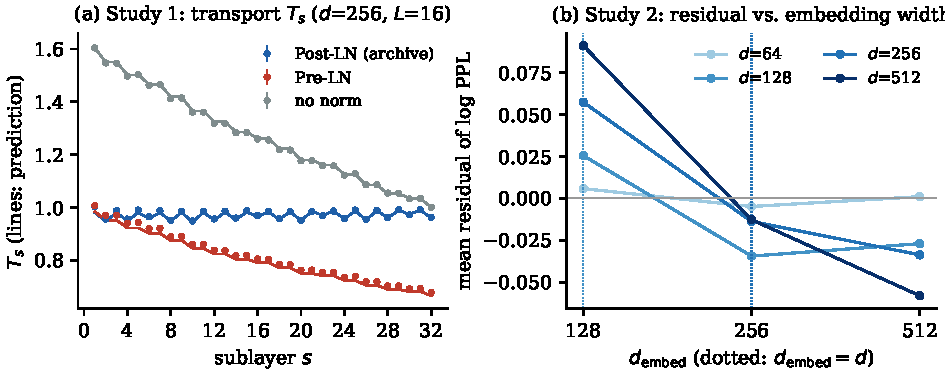
\includegraphics[width=\linewidth]{figure1.pdf}
\caption{(a) Study~1: predicted $T_s$ (lines) and Monte Carlo measurements ($\pm2$ s.e.); Post-LN is nearly flat. (b) Study~2: development residual of log PPL after a within-width fit on log NSC, by embedding width. The benefit of a wider embedding stops near $d_{\mathrm{embed}}=d$ (dotted lines).}
\label{fig:fig1}
\end{figure}

\section{Study 2: capacity of the embedding path}
\textbf{Evidence from data (development only).} Within each width, the residual of log PPL after log projection parameters correlates strongly with the embedding width $d_{\mathrm{embed}}$ (Spearman $-0.01$, $-0.66$, $-0.72$, $-0.87$ for $d=64$ to 512). $d_{\mathrm{embed}}\in\{128,256,512\}$ is assigned independently of the layer configuration (within-width Spearman with projection parameters between $-0.12$ and $0.01$), which makes this a natural experiment. NSC ignores the embedding; total parameter count includes it but counts the $\sim$50k-row tables entry by entry, which ranks models poorly ($\rho=0.73$).

\textbf{Mechanism.} In the adaptive embedding~[10], each token reaches the residual stream through its cluster's table $E$ ($v$ tokens $\times$ $w$ columns, $w=d_{\mathrm{embed}}/\text{div}^i$) and a $w\times d$ projection $P$; the tied softmax reuses the same tables. The path $EP$ has rank at most $\min(w,d)$, so a table wider than $d$ should stop helping. Fig.~\ref{fig:fig1}b shows this saturation: at $d=64$ every table is wider than $d$ and width has no effect; at $d=128$ the gain stops after 256 (tail clusters $256/\text{div}^i$ still fit); at $d=512$ it continues to 512. To score the path we use Study~1's result that Post-LN removes $P$'s overall scale, and take $P$ variance-preserving, $\mathcal N(0,1/w)$. Since $v\gg w$ ($w/v\le0.05$), $E^\top E\approx\sigma^2vI$, so $EP$ has the spectrum of a $w\times d$ matrix with entries $\mathcal N(0,\sigma^2v/w)$:
\begin{equation*}
S_{\text{v3}}=S_0+\textstyle\sum_{\text{tables}}\psimp\bigl(w,\,d,\,\sigma\sqrt{v/w}\bigr),
\end{equation*}
counting each tied table once (a $\text{div}=1$ table with $d_{\mathrm{embed}}=d$ has no projection and contributes $\psimp(v,d,\sigma)$). The ablation removes the embedding term, which recovers NSC exactly. Table shapes reproduce the archive's embedding parameter counts exactly for all 200 models. The formula matches Monte Carlo spectra of $EP$ within 0.4\% RMS over all 60 table shapes in the panel, whereas the literal product at $\sigma=0.02$ is negligible: the score relies on scale invariance, not on raw initial spectra. In a controlled pair with identical layers ($d=256$, $L=6$), NSC ties at 1610.9 for $d_{\mathrm{embed}}=128/256/512$, while $S_{\text{v3}}$ gives 2050.5, 2391.0 and 2323.9: it saturates at $d_{\mathrm{embed}}=d$, where a table without projection scores slightly higher.

\section{Results on development and held-out final architectures}
\begin{table}[t]
\centering
\caption{Spearman $\rho$ with negative PPL; final Kendall $\tau_b$, size-controlled $\tau_b$ (same $d$, total parameters within 10\%; 185 overlapping pairs) and within-width $\rho$. No method below has score ties.}
\label{tab:rank}
\begin{tabular}{lcccccc}
\toprule
& Dev & \multicolumn{5}{c}{Final (held out)} \\
\cmidrule(lr){2-2}\cmidrule(lr){3-7}
Score & $\rho$ & $\rho$ & $\tau_b$ & ctl $\tau_b$ & $\rho_{d=64/128/256}$ & $\rho_{d=512}$ \\
\midrule
\textbf{Study 2 (v3)} & \textbf{0.983} & \textbf{0.980} & \textbf{0.886} & \textbf{0.373} & .940/.947/.950 & \textbf{0.749} \\
Study 1 (v2) & 0.970 & 0.967 & 0.844 & 0.330 & .919/.917/.896 & 0.659 \\
NSC (ablation) & 0.970 & 0.966 & 0.843 & 0.330 & .919/.917/.896 & 0.659 \\
$l/L$ example & 0.970 & 0.969 & 0.853 & 0.319 & .896/.895/.908 & 0.659 \\
Projection params & 0.970 & 0.964 & 0.841 & 0.308 & .898/.917/.896 & 0.658 \\
Reference FLOPs & 0.968 & 0.965 & 0.842 & 0.330 & .924/.921/.900 & 0.658 \\
Total params & 0.728 & 0.742 & 0.590 & 0.276 & .177/.387/.889 & 0.834 \\
\bottomrule
\end{tabular}
\end{table}

\begin{table}[t]
\centering
\caption{Final-split selection: mean regret in PPL (best of top-$k$ minus best feasible) over 200 tie-break or random trials. Pool sizes 25/57/79/96.}
\label{tab:sel}
\begin{tabular}{lcccccccc}
\toprule
Cap / $k$ & 10M/1 & 10M/3 & 20M/1 & 20M/3 & 30M/1 & 30M/3 & 50M/1 & 50M/3 \\
\midrule
v3, v2, NSC, $l/L$, FLOPs & 0 & 0 & 1.14 & 0.85 & 1.62 & 0.77 & 1.37 & 1.33 \\
Projection params & 0 & 0 & 0.85 & 0.85 & 1.62 & 0.77 & 1.37 & 1.33 \\
Total params & 3.72 & 3.72 & 8.44 & 1.49 & 0 & 0 & 1.13 & 1.13 \\
Random & 12.18 & 3.97 & 15.36 & 6.29 & 15.53 & 5.93 & 15.36 & 5.85 \\
\bottomrule
\end{tabular}
\end{table}

\textbf{Ranking.} The pre-registered hypothesis was that $\rho(\text{v3})>\rho(\text{NSC})$ on the final split with a bootstrap 95\% interval (architectures resampled 5000 times) above zero. It holds: $\Delta\rho=+0.015$ [+0.006, +0.028], replicating the development gain of +0.014 [+0.006, +0.026] (Table~\ref{tab:rank}). The largest gain is within $d=512$ (+0.090), where NSC is weakest and the embedding is the smallest stage relative to the layers. Size-controlled $\tau_b$ rises from 0.330 to 0.373. Removing the bottleneck (adding the full embedding capacity) lowers development $\rho$ to 0.924, so the gain comes from the rank-limited path, not from counting embeddings as such. We predicted that v3 would rank $d=64$ models worse than NSC, as it did on development; on final it ranks them better (0.940 vs 0.919), so this prediction failed and the development weakness may have been noise.

\textbf{Selection.} Budgeted top-$k$ selection is identical for v3 and NSC in all eight cells (Table~\ref{tab:sel}): within a parameter cap, the best models are the largest ones, and v3 changes the order among models of similar size rather than across sizes.

\section{Discussion and limitations}
\textbf{What the scores learn beyond size.} NSC is nearly rank-identical to projection parameters (development Spearman 0.9997); Study~1 shows that residual transport cannot change this under Post-LN. Study~2 adds information that size counts miss: the capacity of a serial stage that every token passes, limited by its rank.

\textbf{Aggregation.} We also tested a series rule, $1/S=1/S_0+2/E$, motivated by the embedding being in series with the residual stack. Pre-registered as likely to fail, it did (development $\rho$ 0.930): $\psimp$ sums measure stored capacity, not per-token throughput, so they cannot enter a bottleneck rule directly. Within residual layers summation is supported; across serial stages the right composition remains open, which bears on NSC's sum-versus-product question.

\textbf{Limitations.} Before freezing v3 we examined several embedding variants on development labels (uncapped, rank-capped, Zipf-weighted, two fitted log forms, two series forms); the chosen formula was fixed from label-free checks before its own development evaluation. The final split was used twice. Capacities describe initialization, not training; the reference model omits relative position attention, dropout and attention non-uniformity. The archive has one outcome per architecture and no seeds, so the reported variability covers architecture resampling and tie-breaking only.

\textbf{Ongoing work.} The project continues towards the final report. Any further analysis will use development data only and will be reported as exploratory; the final split will not be used again.

\textbf{Reproducibility and LLM use.} The repository README lists the environment and every command. Methods are frozen at tags \texttt{v2-frozen} and \texttt{v3-frozen}. Scoring 100 architectures takes about 0.1\,s on an Intel Core Ultra 9 290HX (standard library). Claude (Anthropic) and ChatGPT/Codex (OpenAI) assisted with literature reading, code and drafting. All numbers come from the repository's scripts, and the team is responsible for the content.

\newpage
\textbf{References}

\begingroup\small\setlength{\parskip}{1pt}
[1]~Zhu, Zhao, Lu. Neural Spectral Capacity: Measuring and designing architectures from network specification alone. arXiv:2609.23087, 2026.\par
[2]~Javaheripi et al. LiteTransformerSearch: Training-free neural architecture search for efficient language models. NeurIPS 2022.\par
[3]~Tarnowski, Warchoł, Jastrzębski, Tabor, Nowak. Dynamical isometry is achieved in residual networks in a universal way for any activation function. AISTATS 2019.\par
[4]~Wang et al. DeepNet: Scaling Transformers to 1,000 layers. arXiv:2203.00555, 2022.\par
[5]~Xiong et al. On layer normalization in the Transformer architecture. ICML 2020.\par
[6]~Dong, Cordonnier, Loukas. Attention is not all you need: Pure attention loses rank doubly exponentially with depth. ICML 2021.\par
[7]~Noci et al. Signal propagation in Transformers: Theoretical perspectives and the role of rank collapse. NeurIPS 2022.\par
[8]~Cho, Saul. Kernel methods for deep learning. NeurIPS 2009.\par
[9]~Dai et al. Transformer-XL: Attentive language models beyond a fixed-length context. ACL 2019.\par
[10]~Baevski, Auli. Adaptive input representations for neural language modeling. ICLR 2019.\par
\endgroup
\end{document}
